\chapter{Konzept}
\label{ch:Konzept}
In diesem Kapitel wird nun der Entwurf vorgestellt. Dazu möchten wir als erstes die mögliche Lösungsstrategie unseres Systems anschauen und vertiefen warum wir die nötigen Entscheidungen getroffen haben. Dann werden verschiedene Sichten auf das System gezeigt, die das Veranschaulichen sollen.
\section{Lösungsstrategie}
In diesem Abschnitt werden nun die grundlegenden Entscheidungen und Lösungsansätze unseres Entwurfs vorgestellt. Weiteres Vorgehen in Hinblick auf Implementierung hängt hiervon ab.
%Folgende Abbildung veranschaulicht ein mögliches Lösungskonzept auf Top-Level Ebene des Systems
In den folgenden Technologieentscheidungen werden die Entscheidungen der Architektur festgelegt.  
\subsection{Datenbank}
Die Datenbankkomponente ist mit das Herzstück eines Condition Monitoring Systems. Systeme die lange Speicherzeiten benötigen sind den Anforderungen ungenügend. Da das System eine möglichst hohe Lese- und Schreiblast vorweisen muss, bieten sich Extensible-Record Stores Datenbanken an. Diese sind Erweiterungen der Key-Value Stores indem sie für den Wert eine Struktur (ähnlich dem Schema einer Tabelle) zulassen. Schlüssel sind als Bytearray und der Wert besteht aus Paaren von Spaltenname und -wert. Im Gegensatz zum relationalen Modell gibt es kein fixes Schema. Ein solches System ist zum Beispiel Hypertable, das mit einem geringen Speicherplatzbedarf sich optimal eignet. Nach eigenen Angaben soll das System sich sogar um die Konsistenz der Daten kümmern, während sich viele NoSQL-Datenbanken mit einer vermeintlichen Konsistenz der Daten begnügen. Daher haben wir eine kleine Auswahl an Datenbanksystemen miteinander verglichen. Eine Grundeigenschaft war, dass das System ohne Java auskommt, weshalb Cassandra und HBase wegfallen.
\subsubsection{Orcale Berkeley DB}
Orcale Berkeley DB gibt es schon seit 1994 und wurde je nach Edition in C, C++ oder Java implementiert. Es handelt sich dabei um einen Key-Value Speicher, der XML-Unterstützung bietet, SQL und sekundäre Indexierung kann. Die Datenbank wird nach dem ACID-Prinzip gefüllt und ist trotzdem noch sehr schnell bzw. und mit der richtigen Konfiguration auch komplett parallel nutzbar.
\subsubsection{Redis}
Redis ist eine beliebte Datenbanksoftware, die seit 2009 auf dem Markt ist. Sie ist ein in C geschriebener Key-Value-Speicher, der eine große, aber keine vollständige Konsistenz der Daten verspricht. Dafür ist der zugriff komplett parallel und kann durch einige Einstellungen auch stark konsistent werden. Allerdings ist Konsistenz eine starke Anforderung und verpflichtend für die Datenbank.
\subsubsection{Hypertable für Daten}
Das im März 2016 eingestellte Projekt Hypertable basiert auf BigTable und verteilten Daten. Geschrieben wurde es in C++ und ist ein schemafreies System. Die Vorteile liegen in der sofortigen Konsistenz der Daten und der Möglichkeit gleichzeitig lesen und schreiben zu können. Der große Nachteil ist, dass es keine Updates mehr gibt, da das Projekt nicht fortgesetzt wird. Trotzdem ist diese Software in den Schreibvorgängen am schnellsten, wie folgendes Benchmark zeigt \href{https://wiki.volution.ro/Dehems/Benchmarks/Results}{volution.ro}.
\subsection{SQLite für Benutzerverwaltung}
Für die Benutzer- und Rechteverwaltung haben wir uns für SQLite entschieden, da die Datenbank keine Leistung benötigt, schnell integriert und auch in aller Funktionalität ausreichend ist, da es an sie nur wenige Anfragen gibt.
\subsection{Serialisierung Capn Proto}
Da wir mit einem System arbeiten, das eingehende wie ausgehende Daten, in dem System fachterminologisch als Datenpunkt bezeichnet, verarbeitet und mit programminternen sowie /-externen Einheiten kommuniziert, muss bekanntlich auch eine Serialisierung dieser Daten erfolgen.  Bei einer Reihe zur Verfügung stehender Serialisierungstechnologien ist es für das Produkt nötig die Vor- und Nachteile der jeweils einzelnen abzuwägen. Da es für das System von großer Wichtigkeit ist mit einem möglichst großen Datendurchsatz performant umgehen zu können, können textbasierte Serialisierungstechniken wie JSON, XML, YAML usw. kategorisch abgelehnt werden. Der Grund dafür ist, das im allgemeinen ein zu großer Speicherbedarf benötigt wird, was zur Folge hat, dass die Serialisierungszeit und damit auch die Laufzeit stark ansteigt.\\ 
Eine Möglichkeit die Laufzeit zu verringern wäre eine adhoc single String Technik zu verwenden. Diese muss jedoch redundant für jede Sprache geschrieben werden, was uns in der Portierbarkeit einschränken würde.\\
Die nach unserer Meinung nach beste Lösung für dieses Problem wäre es demzufolge eine schemagesteuerte binäre Serialisierungstechnik zu verwenden. Zum Einsatz soll Capn Proto verwendet werden. Durch dessen flexible Schemadefinition lässt sich im Vergleich zu den anderen Portierbarkeit erhöhen, da dieses Framework den Serialisierungscode anhand der Schemadefinition selbst erzeugt. Die binäre Darstellung der Daten erlaubt zudem eine deutlich effizientere Übertragung der Daten. Capn Proto ist im Vergleich zu Protobuf fast doppelt so schnell, siehe \href{https://github.com/ChrisMacNaughton/proto_benchmarks}{Proto Benchmarks}. Die Bibliotheken sind einfach zu nutzen und in C++ geschrieben.
\subsection{Parallelisierung}
Damit alle Systeme und Komponenten zeitgleich ihre Aufgaben erfüllen können, wird die Software in Micro Services aufgebaut, die unabhängig voneinander parallel arbeiten können.\\
Weitere Vorteile liegen in der unabhängigen Entwicklung, Implementierung und Wartung der einzelnen Bausteine. Allerdings wird dadurch auch ein Load Balancer nötig, der die Ressourcen der Hardware nach den Anfragen auf die einzelnen Prozesse verteilt. 
\subsection{Fehlererkennung}
Pings oder ICMP Request/Replies werden zwar oft genutzt um zu sehen, ob ein Server noch online ist, aber da ICMP betriebssystemspezifisch implementiert ist und in manchen Sicherheitsrichtlinien deaktiviert sein muss, kann man das hier nicht für eine dauerhafte Taktik verwenden. Außerdem erhält man keine Einsicht darüber, ob ein Programm auf der Maschine ausgeführt ist, was in unserem Fall aber wichtig wäre. 
\\
Mit Hilfe von Monitoring kann man die Antwortzeiten und die Uptimes von allen Anwendungen eines Servers abfragen und darstellen. Diese Methode ist zielführender, braucht allerdings eine zusätzliche Schnittstelle, die nicht immer bereitgestellt werden kann. Auch verbraucht sie einige Ressourcen und die Abfrage kann bzw. sollte nicht in zu kurzen Zeitintervallen stattfinden. 
\\
Heartbeat ist eine periodischer Nachrichtenaustausch zwischen einem Prozess und einem Kontrollsystem. Da unsere Anwendung in Echtzeit große Datenmengen bewältigen muss, ist es wichtig, dass der Heartbeat schnell und einfach gesendet und empfangen wird um keine anderen Daten/Datenverarbeitung zu behindern. 
Mit Hilfe von Condition Monitoring kann man zum Beispiel bei einer Maschine aus Sensordaten Schwingungen und Temperaturen erfassen, die evtl. für Ausfälle sorgen. Um das bei unserem Server anzuwenden, muss man die CPU-Temperatur überwachen und ggf. den Serverschrank weiter runterkühlen um Ausfälle zu vermeiden. 
Voting ist nicht nur prozessorlastig, sondern wird am besten auch auf mehreren Geräten gleichzeitig ausgeführt was langsam und kostenintensiv ist, daher verwerfen wir diese Möglichkeit.
\\
Zeitstempel kann man einfach in die Datenbank einpflegen um evtl. fehlerlastige Zeiten herauszufinden und zu löschen oder zu korrigieren. Eine größere Validierung wird wieder zu CPU-lastig und kann daher nicht direkt beim Speichern der Daten durchgeführt werden.
Aus Kostengründen müssen wir auch alle Wiederherstellungsmaßnahmen, die Redundanz beinhalten leider ausschließen, da das Budget zu klein gesetzt wurde. Daraus folgt treten Softwarefehler ein, muss man mit Hilfe von Hotfixes und bei Hardwarefehlern mit einem Austauschgerät arbeiten. Außerdem kann man bei Exceptions, die zur Laufzeit auftreten den jeweiligen Stacktrace mit der dazugehörigen Eingabe an eine Kontrollstelle abspeichern. Sobald eine kritische Anzahl an Exceptions pro Minute/Stunde auftritt muss der Fehler in der Software gepatcht werden. Im Softwaredesignprozess muss dabei darauf geachtet werden, dass Exceptions immer gehandelt werden und das auch in sehr ungewöhnlichen oder gar unmöglichen Fällen um in jedem Szenario handlungsfähig zu bleiben.
\\
Abschließend haben wir uns für eine Kombination aus Condition Monitoring, Exception Handling und Zeitstempel entschieden, weil diese kaum Leistung benötigen und Kosten verursachen. Hotfixes für Ausfälle sind gerade im Pilotbetrieb erstmal günstiger als redundante Hardware und komplexe Monitoringtools. Diese können bei Bedarf in einer späteren Variante auf besserer Hardware eingebaut werden.
\section{Bausteinsicht}
Unsere Hardware ist ein Raspberry Pi aus der ersten Generation, der im Serverschrank über Fastethernet ans Produktionsnetzwerk angebunden ist. Außerdem hat er RS485, USB und CAN-Ports um mit allen Geräten kommunizieren zu können.\\
Die folgende Grafik zeigt den ersten Überblick über das System, welches in ihre Einzelheiten und ihre Micro Services zerlegt ist.
\begin{figure}[h]
	\centering
	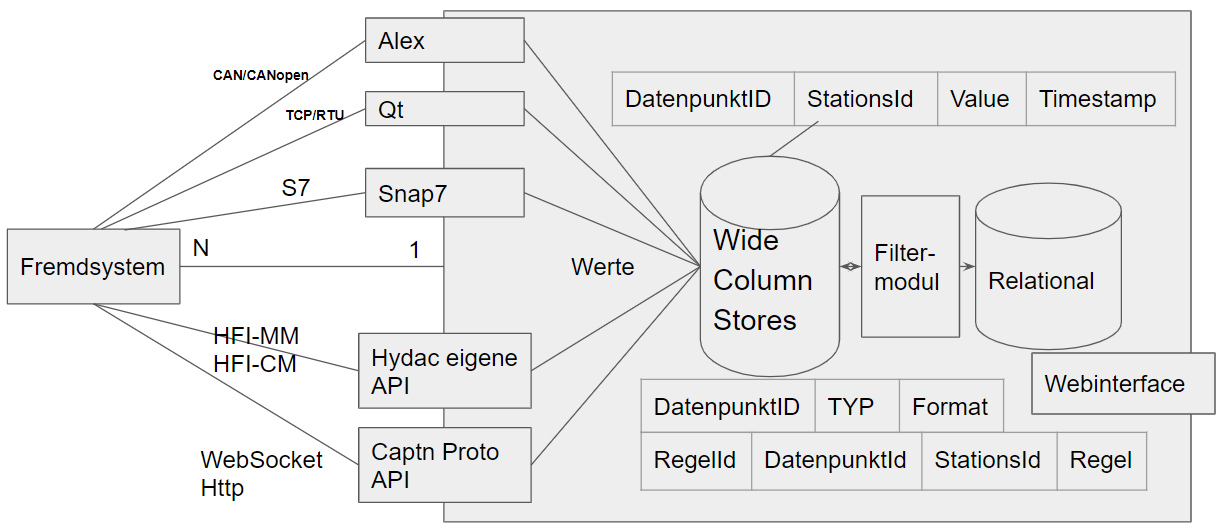
\includegraphics[width=1.0\textwidth]{Graphics/blackbox1.png}
	\caption{Erste Ebene}
	\label{fig:erste_ebene}
\end{figure}
Damit die die vielen Fremdsysteme und Maschinen mit unserer Software kommunizieren können, benötigen wir Implementierungen aller Protokolle in C++. Für CAN bzw. CANopen hat Alex eine Bibliothek in seiner Bachelorarbeit geschrieben. Für TCP/RTU nutzen wir Qt, für S7 gibt es Snap7. Die Hydac hat ihre eigene API und Bibliothek für die eigenen HFI-MM und HFI-CM Protokolle. Zu guter Letzt serialisieren wir WebSocket und HTTP mit Capn Proto. Alle Bibliotheken ermöglichen das einfache Abspeichern in den Wide-Column-Store oder bereiten es zumindest vor. Dafür werden eine DatenpunktID und StationsID der Maschine mit dem Wert und dem Zeitstempel gespeichert. Da diese Daten komplett ungeprüft in die Datenbank einfließen, muss ein weiterer Baustein alle Einträge überprüfen und Messfehler oder kritische Werte direkt in der Weboberfläche anzeigen. Dass die Überprüfung eventuell etwas langsamer als der Datenstrom in die Datenbank sein kann, ist an sich nicht schlimm, da die Anwendung in Produktionspausen aufholen und die noch ungeprüften Daten währenddessen verarbeitet.\\
In der relationalen Datenbank befinden sich dann die DatenpunktIDs mit ihren Typen und Formaten, damit man ein Schema zur Darstellung im Interface hat. zusätzlich zu den Nutzer- und Rechtedaten gibt es auch noch eine Tabelle, die Regeln für die Datenpunkte abbildet.\\
\begin{figure}[h]
	\centering
	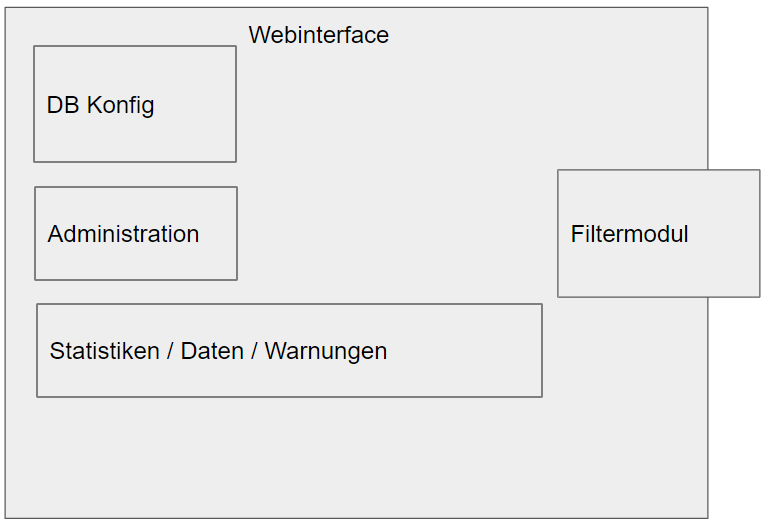
\includegraphics[width=0.7\textwidth]{Graphics/blackbox2.png}
	\caption{Zweite Ebene}
	\label{fig:zweite_ebene}
\end{figure}
Das Webinterface hat zu beiden Datenbanken eine Verbindung und kann auch die API des Filtermoduls mitbenutzen. In der Nutzeroberfläche wird zwischen einem administrativem und einem anwendungsspezifischen Teil unterschieden. In letzterem werden nur Daten und Statistiken aufbereitet angezeigt, während die Rechtevergabe und Feineinstellung in der Administratoroberfäche stattfindet. 
\section{Laufzeitsicht}
\section{Verteilungssicht}